\chapter{SRD}

\section{Introducción}

En este capitulo se explicará el funcionamiento del diodo SRD.  Estos pertenecen
a una familia de dispositivos de juntura denominada junturas de almacenamiento
de carga \cite{moll1962}. Estos dispositivos se caracterizan por su
característica de recuperación inversa.

Se empezará explicando principios básicos de funcionamiento de diodos de
juntura, luego el proceso de recuperación inversa en un diodo, y luego una
descripción del diodo SRD y sus modelos de simulación.

\section{Introducción a diodos}

Un diodo es un dispositivo electrónico caracterizado por una relación
tensión-corriente asimétrica, presentando una impedancia muy baja en un sentido
de circulación de corriente y muy alta en el opuesto. Por esta característica
tienen aplicaciones como rectificadores, tanto en circuitos de potencia como de
comunicaciones.

\subsection{Física de la juntura}
\label{sec:junction_physics}

\begin{figure}
    \centering
    \begin{subfigure}[b]{0.45\textwidth}
        \centering
        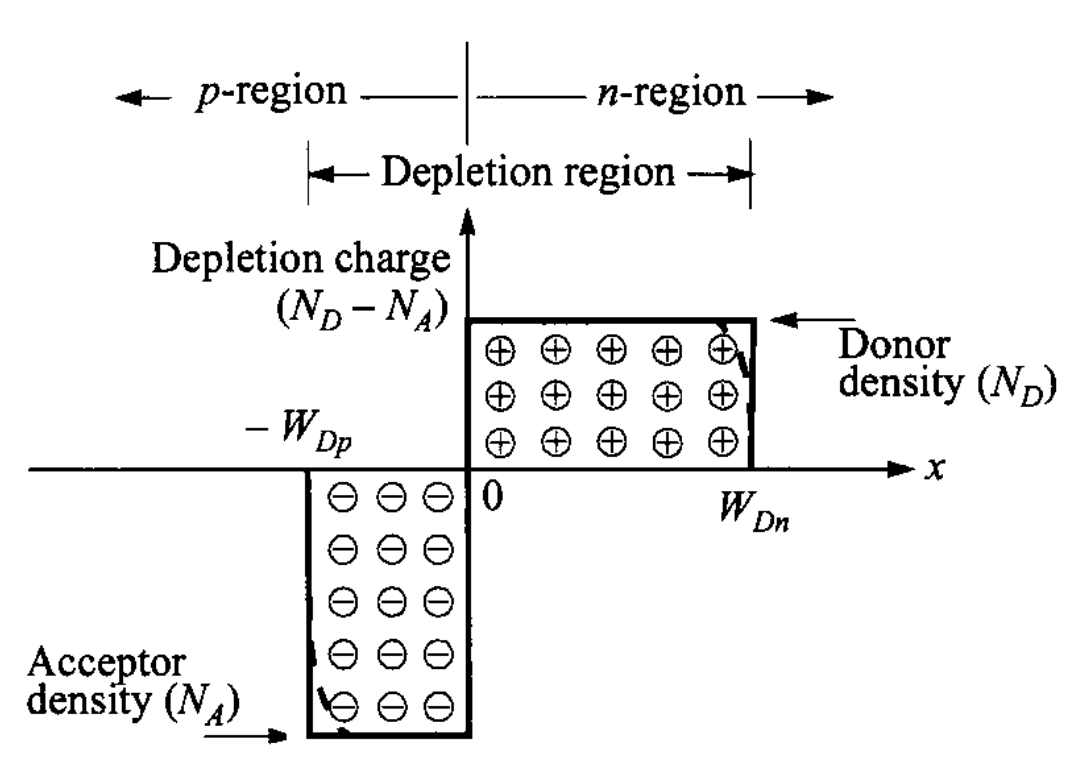
\includegraphics[width=0.8\textwidth]{images/pn_junction_equilibruim.png}
        \caption{Juntura PN en equilibrio.}
        \label{fig:pn_junction_equilibruim}
    \end{subfigure}
    \hfill
    \begin{subfigure}[b]{0.45\textwidth}
        \centering
        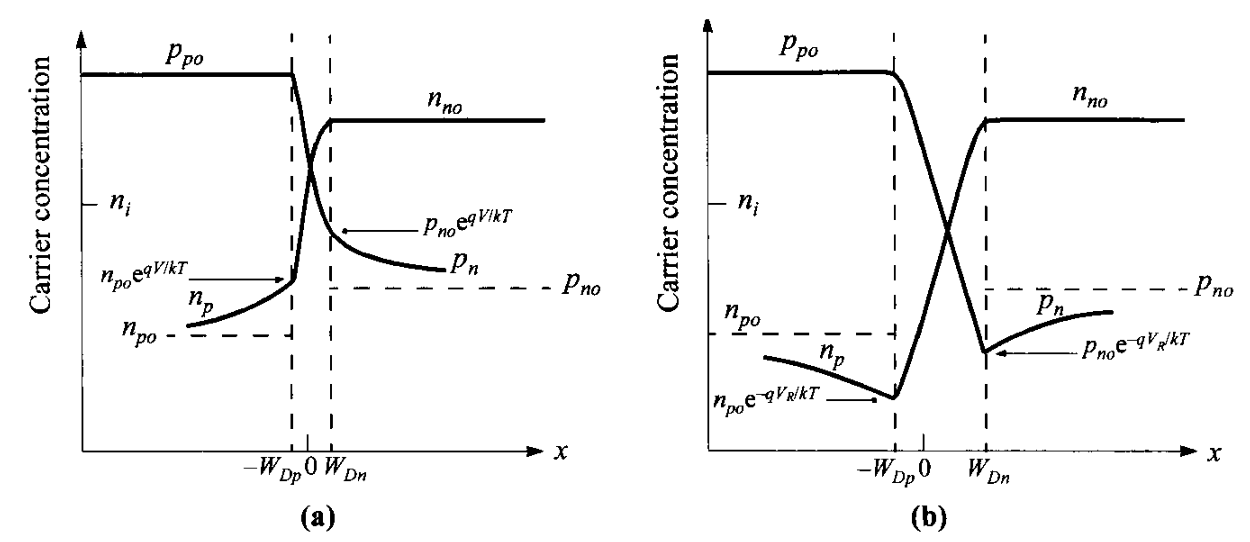
\includegraphics[width=\textwidth]{images/pn_junction_under_bias.png}
        \caption{Juntura PN bajo polarización a) directa y b) inversa.}
        \label{fig:pn_junction_under_bias}
    \end{subfigure}
    \caption{Juntura PN en equilibrio y en polarización. Tomadas de
    \cite{Sze2006}.}
    \label{fig:pn_junction_plots}
\end{figure}

El funcionamiento del diodo se basa en una juntura. Esta puede ser
semiconductor-semiconductor, como en un diodo de juntura pn, semiconductor-metal
como en un diodo Schottky, semiconductor-semiconductor-semiconductor como en un
diodo PIN, o demás variaciones. Los principios físicos de funcionamiento de toda
esta familia de dispositivos se basa en la física de la densidad de portadores
en estos materiales y sus distintos fenómenos de transporte
\cite{neamen2012semiconductor}.

Existen dos fenómenos de transporte en una juntura: la difusión y el arrastre.
La primera se debe al fenómeno físico de difusión, en el que un gradiente de
densidad resulta en una corriente desde las zonas con mayor concentración a las
de menor. La corriente de arrastre se debe al campo eléctrico existente en la
juntura.

\subsubsection{Juntura en equilibrio}
\label{sec:pn_junction_equilibruim}

En una juntura pn en equilibrio, las corrientes de difusión y arrastre se
encuentran perfectamente balanceadas. Debido a los gradientes de concentración
de portadores en la juntura, alrededor de la misma se forma una zona vacía de
portadores, denominada zona desierta o zona de carga espacial. En esta zona,
debido a la ausencia de portadores minoritarios, se desarrolla una densidad de
carga, debido a los iones no compensados. Esta zona resulta en un campo
eléctrico que a su vez genera una corriente de arrastre que compensa a la de
difusión.

Entonces, el ancho de esta zona desierta dependerá del dopaje en ambos
materiales y de la geometría de los mismos, dado que el mismo es el necesario
para compensar la corriente de difusión. En la figura
\ref{fig:pn_junction_equilibruim} se observa un esquema de la situación. En
ambos materiales se desarrollan zonas desiertas, de anchos $W_{Dp}$ y $W_{Dn}$
con carga total de $W_{Dp} \cdot N_A$ y $W_{Dn} \cdot N_D$.

Es una caso de interés el de una juntura muy asimétrica, en la que $N_A >> N_D$
o $N_A << N_D$. Por la neutralidad de carga, las cargas almacenadas en cada zona
desierta $Q_N$ y $Q_P$ deben ser iguales. En el caso de una juntura muy
asimétrica, esto resulta en el ancho de la zona fuertemente dopada siendo casi
cero, es decir $W_{Dp} \approx 0$ si $N_A >> N_D$ o $W_{Dn} \approx 0$ si $N_D
>> N_A$.

La aproximación de juntura muy asimétrica es de interés ya que puede ser
aplicada a cierto tipo de junturas, como la metal-semiconductor o la
semiconductor dopado-semiconductor intrínseco. La primera aplica para diodos
Schottky mientras que la segunda es de utilidad en diodos PIN y SRD.

\subsubsection{Juntura polarizada}

Una vez que se aplica una tensión $V_D$ entre los terminales del dispositivo, el
ancho de esta zona varía, descompensado el equilibrio entre las corrientes de
difusión y arrastre. Una tensión $V_D > 0$ resulta en un achicamiento de la zona
desierta, una reducción del campo eléctrico y una corriente neta de difusión.
Para $V_D < 0$, la zona de vaciamiento aumenta, aumentando el campo eléctrico y
resultando en una corriente neta de arrastre.

En la figura \ref{fig:pn_junction_under_bias} se observa como varían las
densidades de portadores y el ancho de la zona desierta. Para tensiones
positivas (polarización directa), el ancho de la zona desierta disminuye y las
densidades de portadores minoritarios están en exceso de las de equilibrio, y
para inversa, la zona desierta se incrementa y las densidades caen por debajo de
las de equilibrio.

Este exceso de portadores minoritarios para polarización directa resulta en una
corriente considerable, y la baja densidad en inversa en una corriente casi
nula. Este es el efecto mencionado anteriormente de asimetría en la conducción
de corriente.

Según el valor de $V_D$ se determinan dos regímenes de operación distintos: el
régimen de directa, en el que la corriente es considerable, y régimen de
inversa, en el que la corriente es prácticamente nula.

\subsection{Relación I-V}

Cómo fuese explicado en la sección \ref{sec:junction_physics}, existe una
relación entre la tensión $V_D$ aplicada entre los terminales del diodo y la
corriente $I_D$ por el mismo. Se explicó cualitativamente cómo tensiones
positivas resultan en circulación de corrientes y negativas en corriente nula.
Cuantitativamente esta relación puede expresarse de la siguiente manera
\cite{neamen2012semiconductor}

\begin{equation}
    I = I_S \left( e^{\frac{V_D}{V_T}}-1\right).
\end{equation}

El parámetro $I_S$ depende del diseño del diodo, y la tensión $V_T$ es una
tensión fuertemente dependiente de la temperatura. Para diodos de silicio, esta
expresión suele ser aproximada a orden 0 como una corriente $I=0$ para $V<
\qty{0.6}{\volt}$, y para corrientes $I>0$ una tensión fija de $V =
\qty{0.6}{\volt}$.

Esta es una relación estática, es decir, la relación obtenida una vez
extinguidos todos los transitorios. Linealizando a partir de un cierto punto de
operación estático, es posible desarrollar un modelo dinámico de pequeña señal.
Este está compuesto por una resistencia $r_D$, una capacidad de difusión $c_D$ y
una capacidad de juntura $C_j$. La capacidad de difusión tiene su fundamento
físico en el cambio en la carga almacenada en el dispositivo por el proceso de
difusión, y la capacidad de juntura en la variación del ancho de la zona
desierta con la tensión $V_D$. Al variar el ancho, varía la carga almacenada en
la misma, por lo que tiene un efecto capacitivo. En la figura
\ref{fig:diode_model} se observa el modelo de pequeña señal.

\begin{figure}
    \centering
    \begin{subfigure}[b]{0.45\textwidth}
        \centering
        \begin{adjustbox}{scale=0.8}
            \begin{circuitikz}[american]
                \draw (0,4) to[open] (0,3);
                \draw (0,3) to[D*, l=$D$, v=$V_D$, i=$I_D$] (0,1);
                \draw (0,1) to[open] (0,0);
            \end{circuitikz}
        \end{adjustbox}
        \caption{Tensión y corriente en un diodo.}
    \end{subfigure}
    \hfill
    \begin{subfigure}[b]{0.45\textwidth}
        \centering
        \begin{adjustbox}{scale=0.8}
            \begin{circuitikz}[american]
                \draw (-1,4) to[open, v=$V_D$] (-1,0);
                \draw (2,4) to[short, i=$I_D$] (2,3);
                \draw (0,3) to[short] (4,3);
                \draw (0,3) to[R, l=$R_D$] (0,1); % Resistor R_D
                \draw (2,3) to[C, l=$C_D$] (2,1); % Capacitor C_D
                \draw (4,3) to[C, l=$C_j$] (4,1); % Capacitor C_j
                \draw (0,1) to[short] (4,1);
                \draw (2,1) to[short, i=$I_D$] (2,0);
            \end{circuitikz}
        \end{adjustbox}
        \caption{Modelo de pequeña señal del diodo.}
    \end{subfigure}
    \caption{Modelo de diodo.}
    \label{fig:diode_model}
\end{figure}

Para modelar el comportamiento dinámico de gran señal, es necesario contemplar
la física de las transiciones entre los estados de directa e inversa. La
transición de directa a inversa se denomina proceso de recuperación inversa, y
es el proceso en que el diodo SRD es distintivo. A continuación se analizará en
detalle la física de esta transición.

\section{Proceso de recuperación inversa}

En la figura \ref{fig:diode_reverse_recovery} se observa el proceso de
recuperación inversa de un diodo. El mismo se encuentra polarizado en directa
con una corriente $I_f$, y en el instante $t_0$ se aplica una corriente negativa
$I_r$. Durante un tiempo $t_s$, denominado tiempo de almacenamiento
(\textit{storage time} en inglés), el diodo permanece en un estado de baja
impedancia, conduciendo corriente. Luego de este tiempo, durante $t_t$ ($t_2$ en
la figura) se da el tiempo de transición (\textit{transition time} o
\textit{decay time} en inglés).  Durante este tiempo, la impedancia de la
juntura transiciona de bajo a alto, interrumpiendo la conducción de corriente.
El tiempo total $t_s+t_t$ es denominado tiempo de recuperación $t_{rr}$.

\begin{figure}[t]
    \centering
    \begin{subfigure}[b]{0.45\textwidth}
        \centering
        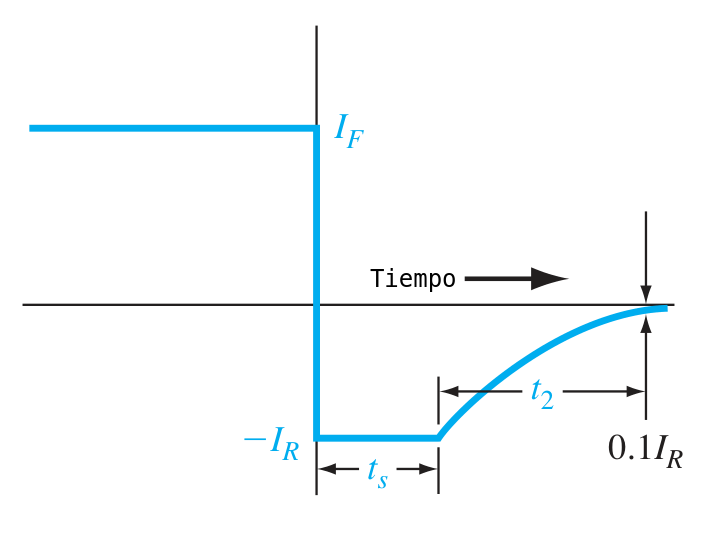
\includegraphics[width=0.6\textwidth]{images/diode_reverse_recovery.png}
        \caption{Recuperación inversa de un diodo. Tomado de
        \cite{neamen2012semiconductor}}
        \label{fig:diode_reverse_recovery}
    \end{subfigure}
    \hfill
    \begin{subfigure}[b]{0.45\textwidth}
        \centering
        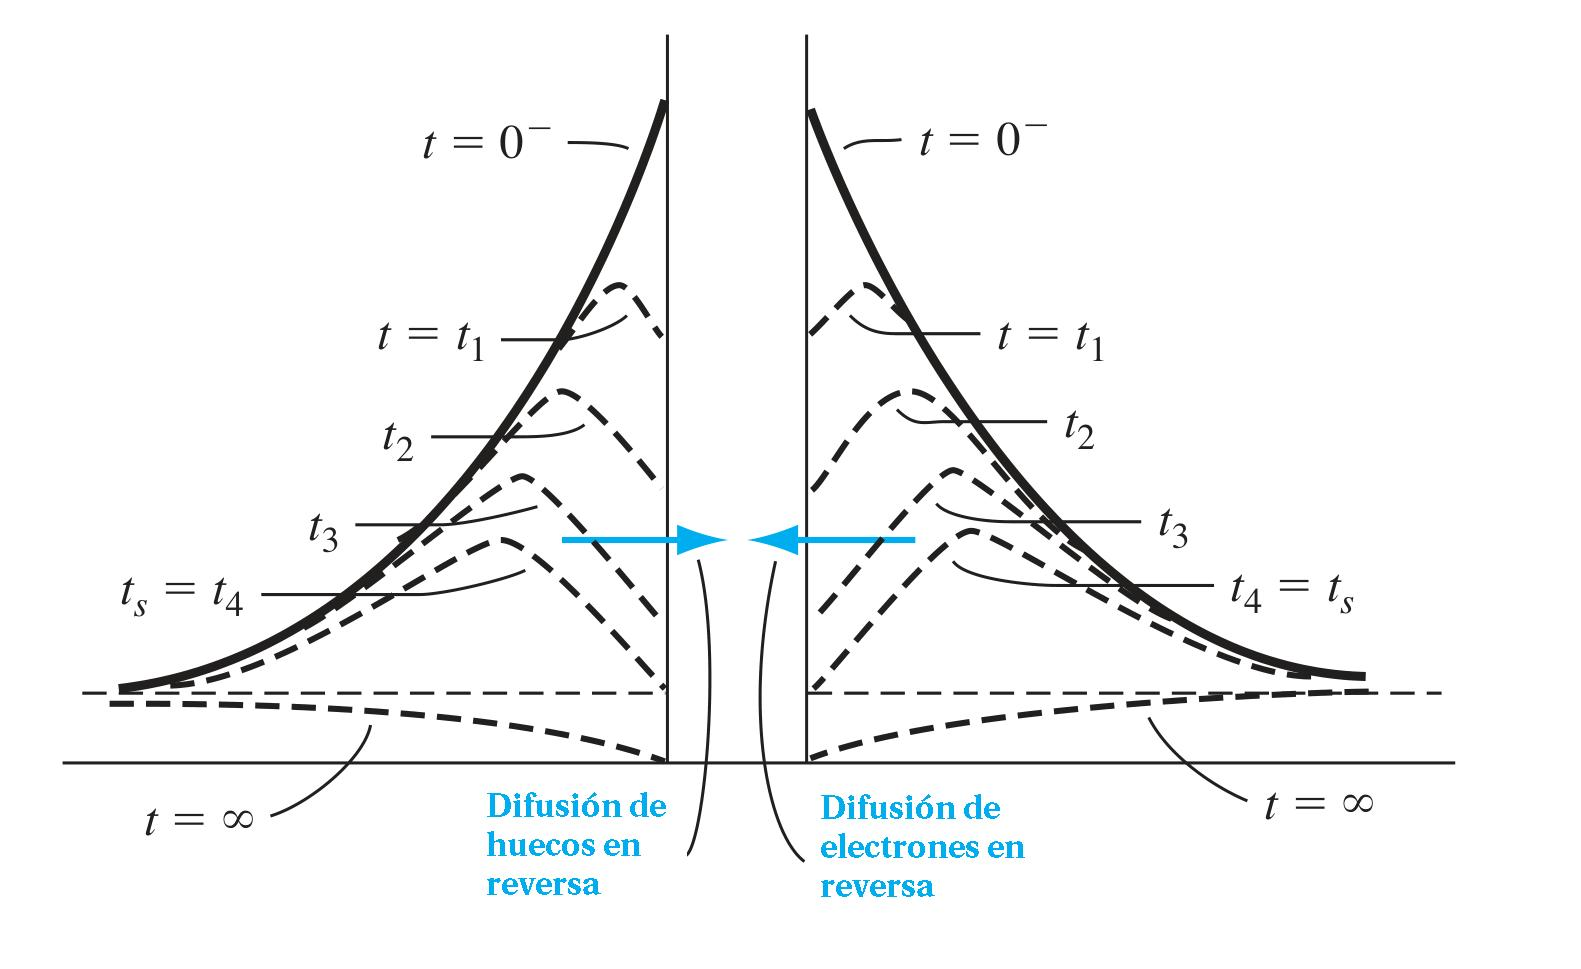
\includegraphics[width=\textwidth]{images/carrier_concentrations_turnoff.jpg}
        \caption{Evolución de densidad de portadores en el proceso de
        recuperación inversa. Tomado de \cite{neamen2012semiconductor}}
        \label{fig:carrier_concentrations_turnoff}
    \end{subfigure}
    \caption{Proceso de recuperación inversa en un diodo.}
    \label{fig:pn_reverse_recovery_plots}
\end{figure}

Cada una de estas fases está relacionada a distintos procesos físicos que se dan
en la juntura. Cuando el diodo se encuentra en directa, la zona de vaciamiento
se reduce, resultando en un menor campo eléctrico, y una corriente neta de
difusión. Este mecanismo resulta en densidades de portadores minoritarios en los
extremos de la zona de vaciamiento proporcionales a $exp(V/V_t)$, resultando en
una inyección de portadores minoritarios en ambas partes de la juntura. Entonces
el diodo en directa tiene un exceso de portadores minoritarios.
\cite{neamen2012semiconductor}

El tiempo de almacenamiento $t_s$ está asociado al tiempo que demora la
corriente reversa $I_r$ en remover el exceso de portadores minoritarios de la
zona de vaciamiento. El tiempo de almacenamiento termina una vez que la densidad
de portadores minoritarios en los extremos de la zona de vaciamiento caen a sus
valores de equilibrio térmico.

Una vez terminado el tiempo de almacenamiento, las densidades de portadores
minoritarios en los extremos de la zona de vaciamiento cayeron a sus valores de
equilibrio térmico, pero en las zonas P y N todavía se encuentra una densidad de
portadores mayor a la de una juntura en reversa. El tiempo de transición $t_t$
esta asociado al tiempo que demoran estas densidades en caer a sus valores de
estado estacionario.

En la figura \ref{fig:carrier_concentrations_turnoff} se observa la evolución
temporal de las densidades. Se observa que en $t=0^-$ las densidades en los
extremos de la zona de vaciamiento están en sus valores máximos, y en $t_4=t_s$
caen a sus valores de equilibrio térmico. Sin embargo, en este instante las
densidades en el cuerpo de la juntura no están en sus valores de estado
estacionario $t=\inf$.

\section{Diodos de almacenamiento de carga}
\label{sec:charge_storage_diodes}

En \cite{moll1962} de desarrolla la teoría de los diodos de almacenamiento de
carga. Estos se caracterizan por su particular comportamiento de recuperación
inversa.

En un diodo de juntura usual, tanto el tiempo de almacenamiento como el de
transición tienen un orden de magnitud similar al tiempo de vida de los
portadores minoritarios $\tau_m$, o MCL del inglés \textit{Minority Carrier
Lifetime}. La característica distintiva de los diodos de almacenamiento de
carga, es que el tiempo de almacenamiento mantiene su orden de magnitud de
$\tau_m$, pero el tiempo de transición $t_t$ es mucho menor. \cite{moll1962}

En aplicaciones de conmutación de señal, es deseado que el tiempo de
recuperación $t_{rr}$ sea lo menor posible. Esto minimiza las pérdidas de
potencia y maximiza la frecuencia de operación. En aplicaciones de generación de
pulsos o multiplicación de frecuencia, no es deseado un $t_{rr}$ mínimo.

La combinación de tiempo de almacenamiento $t_s$ finito y tiempo de transición
$t_t$ muy corto es de utilidad en aplicaciones de generación de pulsos o
multiplicación de frecuencia. En la figura
\ref{fig:charge_storage_diode_waveforms} se observa el comportamiento de un
diodo de este tipo y uno con tiempo de recuperación 0.

En el caso del diodo llave ideal, la señal de salida sigue a la entrada cuando
esta es positiva, y es nula cuando la entrada es negativa, es decir, es un
rectificador ideal. En el caso de un diodo de almacenamiento de carga, hay un
tiempo de almacenamiento finito y comparable al período de la señal de entrada,
por lo que la señal de salida sigue a la entrada mientras esta es negativa.
Terminado el período de almacenamiento, el rápido tiempo de transición resulta
en un flanco de amplitud considerable y muy corto. Esta característica permite
generar pulsos ultra cortos o harmónicos altos de la señal de entrada.

\begin{figure}[t]
  \centering
    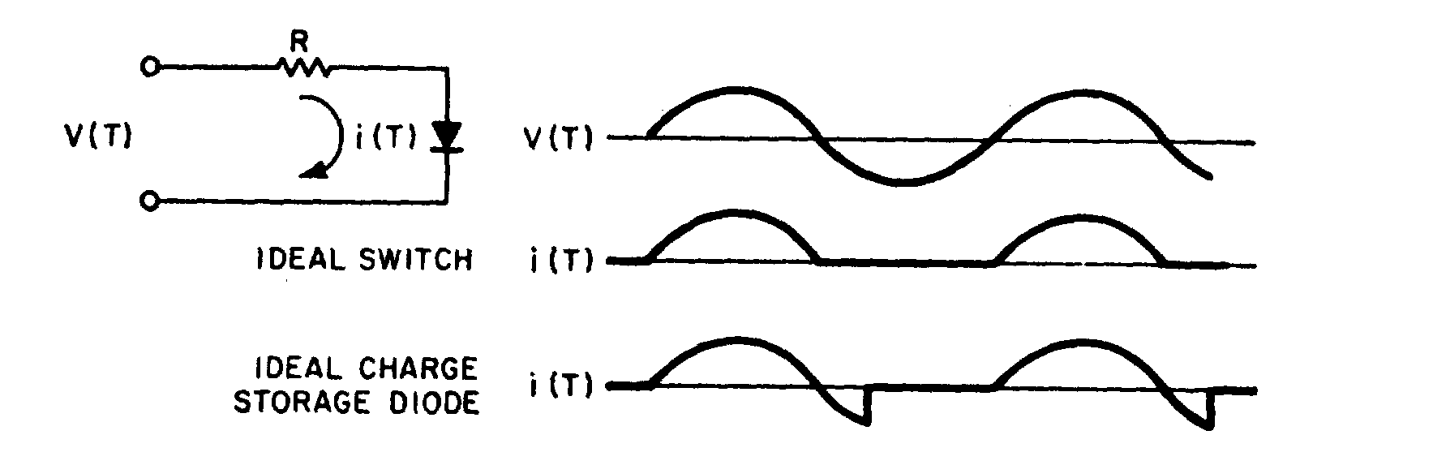
\includegraphics[width=0.4\textwidth]{images/charge_storage_diode_waveforms.jpg}
    \caption{Formas de onda en rectificadores. Tomado de \cite{moll1962}.}
    \label{fig:charge_storage_diode_waveforms}
\end{figure}

Los diodos de almacenamiento de carga implementan estas características de gran
tiempo de almacenamiento $t_s$ y tiempo de transición corto $t_t$. El tiempo de
almacenamiento prologando se obtiene implementando un MCL $\tau_m$ máximo
posible para el proceso de fabricación. El tiempo $t_t$ mínimo, se logra con un
diseño de diodo que resulte en una distribución de portadores en directa tal que
la mayoría de las cargas se encuentren muy cerca de la zona de vaciamiento. De
esta manera, una vez que las cargas de la zona de vaciamiento se remueven,
prácticamente no quedan cargas en el dispositivo, minimizando el tiempo de
transición $t_t$.

En \cite{moll1962} se demuestra que, siendo $x_0$ la distancia desde el centro
de la juntura al centro de gravedad de la distribución de portadores, el tiempo
$t_t$ será proporcional a $x_0^2/D$, con $D$ la constante de difusión promedio.
Se demuestra también que a mayor carga almacenada en el diodo, mayor es el valor
de $x_0$. Es decir, un incremento de la carga trae un incremento en la
dispersión de la distribución de la carga con respecto al centro de la juntura.
Es entonces que existe una relación inversa entre carga almacenada $Q$ y tiempo
de transición $t_t$: a mayor carga $Q$, mayor $x_0$ y mayor $t_t$.

Otra limitante para $t_t$ es la capacidad de la juntura $C_j$. Esta capacidad
debe ser descargada en la transición, por lo que mayores valores de $C_j$
resultan en un $t_t$ más lento.

$C_j$ y la carga almacenada $Q$ están relacionadas a través del área de la
juntura $A$. La capacidad $C_j$ varía directamente con el área mientras que la
carga inversamente. Es decir, mayor área, mayor capacidad y menor carga por
unidad de área. Entonces, existe un compromiso en el diseño del diodo con
respecto al área: mayores áreas resultan en menor densidad de carga pero mayor
capacidad y viceversa. \cite{moll1962}

\section{Diodo SRD}
\label{sec:srd_diode}

El diodo SRD, del inglés \textit{Step Recovery Diode}, diodo de recuperación en
escalón, es un tipo de diodo de almacenamiento de carga, con las características
de los mismos descriptas en la sección \ref{sec:charge_storage_diodes}.

\subsection{Física del dispositivo}

El diodo es un un diodo PIN, es decir, un semiconductor intrínseco, la capa I,
entre dos semiconductores P y N. En la figura \ref{fig:srd_diode_structure} se
observa la estructura del mismo. La característica que diferencia al diodo SRD
de los diodos PIN usuales con aplicaciones en RF, es que en el SRD la capa I es
muy fina, entre \qty{0.5}{\micro\meter} y \qty{4}{\micro\meter}, mientras que en
un diodo PIN el rango es entre \qty{50}{\micro\meter} y
\qty{1000}{\micro\meter}.

El ancho de la capa I del diodo SRD le permite tener un MCL relativamente largo
y un tiempo de transición relativamente corto, características descriptas en
la sección \ref{sec:charge_storage_diodes} deseables para aplicaciones de generación de pulsos.

La capa I logra un dispositivo con un MCL considerable. Para lograr un tiempo de
transición lo más corto posible, como fuese explicado en la sección
\ref{sec:charge_storage_diodes}, es necesario que la mayoría de los portadores
minoritarios se encuentren alrededor de la zona de vaciamiento. Esto se logra
realizando un diodo $p^+in^+$, donde las zonas $p$ y $n$ están fuertemente
dopadas. Esto resulta en una almacenamiento de portadores en la zona intrinseca
$i$, y barreras de potencial que fuerzan a los portadores a mantenerse en la
zona $i$.

La capa I tiene un efecto importante sobre la capacidad de juntura. Debido a que
las junturas $p^+i$ y $in^+$ son del tipo fuertemente asimétricas, como fuese
explicado en la sección \ref{sec:pn_junction_equilibruim}, la zona de
vaciamiento se encuentra prácticamente confinada a la región I. Debido a esto,
la región de vaciamiento es esencialmente invariable con la tensión $V_D$. Esto
resulta en una capacidad de juntura $C_j$ independiente de la tensión y muy
chica \cite{maas2003} \cite{Sze2006} \cite{moll1969}.

\begin{figure}[t]
    \centering
    \begin{subfigure}[b]{0.45\textwidth}
        \centering
        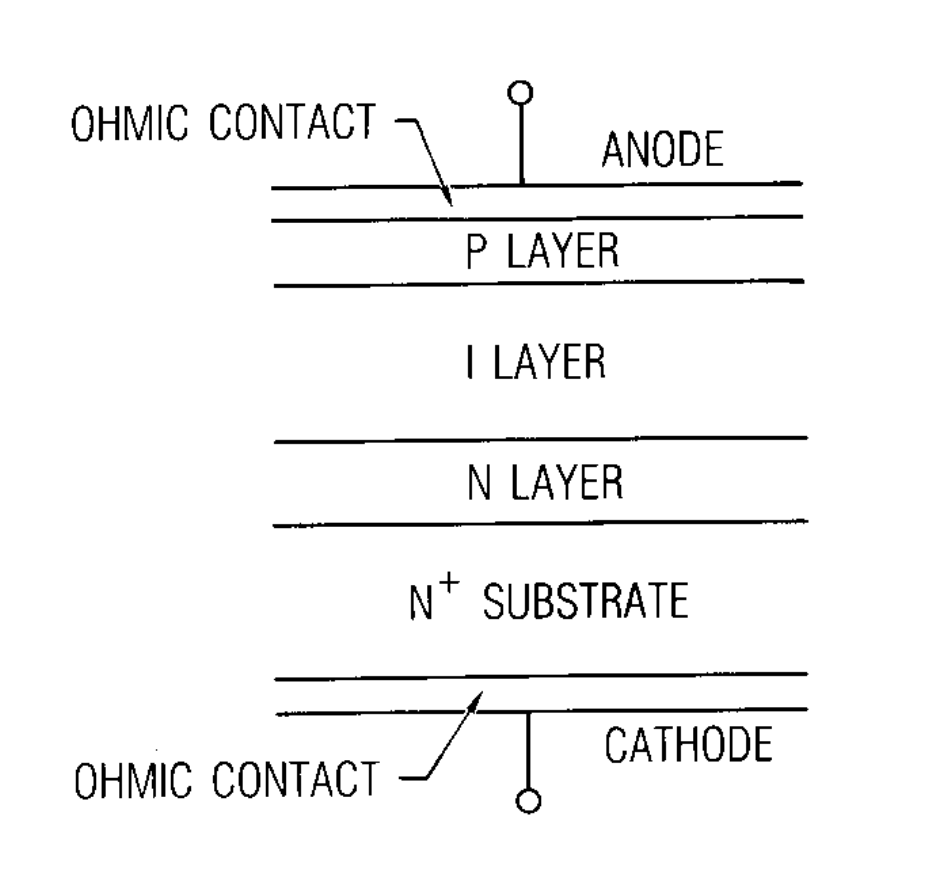
\includegraphics[width=0.8\textwidth]{images/srd_diode_structure.jpg}
        \caption{Estructura física del diodo SRD. Tomado de \cite{maas2003}.}
        \label{fig:srd_diode_structure}
    \end{subfigure}
    \hfill
    \begin{subfigure}[b]{0.45\textwidth}
        \centering
        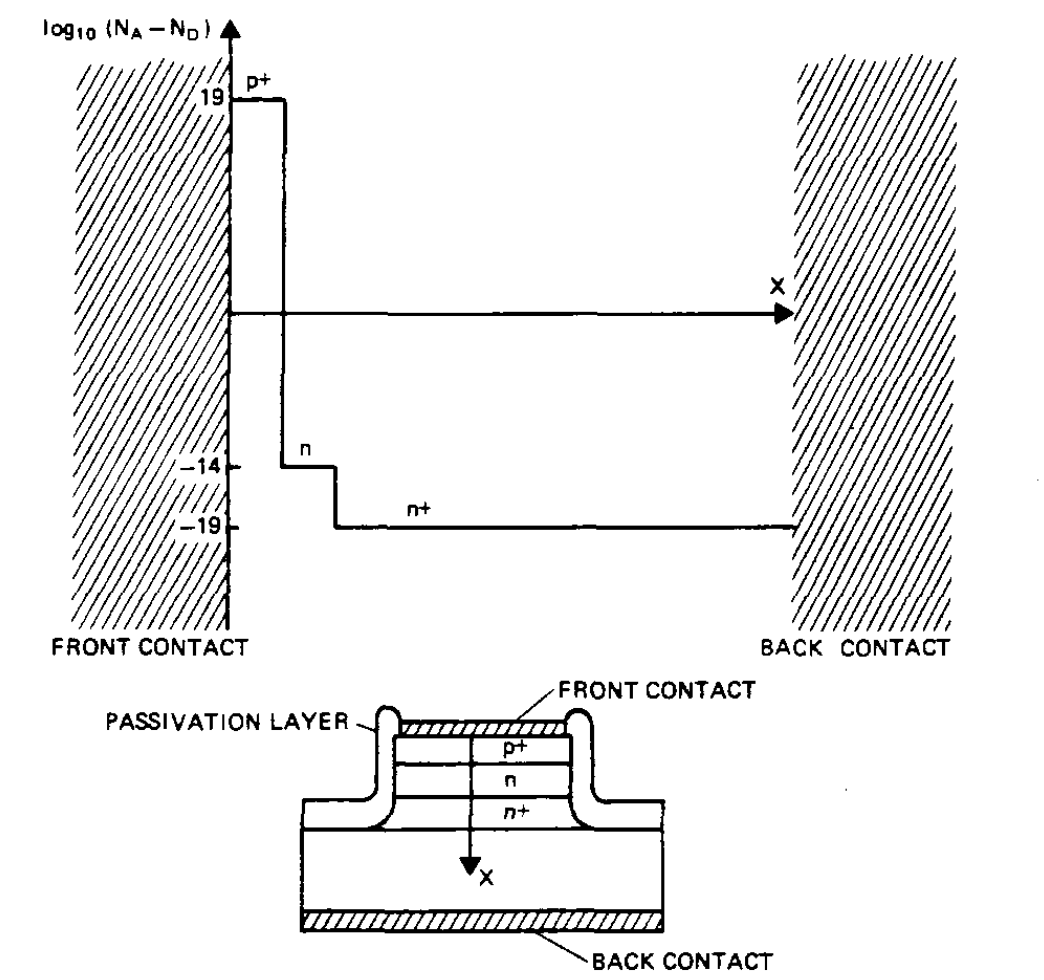
\includegraphics[width=0.8\textwidth]{images/srd_impurity_profile.jpg}
        \caption{Densidad de dopaje en SRD. Tomado de \cite{moll1969}}
        \label{fig:srd_impurity_profile}
    \end{subfigure}
    \caption{Geometría y dopaje en un SRD.}
    \label{fig:srd_gemotry_and_doping}
\end{figure}

\subsection{Proceso de recuperación}

Analizaremos ahora las características del proceso de recuperación en un diodo
SRD.

Para encontrar el tiempo de almacenamiento $t_s$ en un diodo SRD, puede
plantearse la ecuación de continuidad de carga \cite{moll1962} \cite{moll1969}

\begin{equation}
    \frac{dQ}{dt} = I-\frac{Q}{\tau_m}
\end{equation}

Esta ecuación contempla la inyección/remoción de carga mediante la corriente
externa $I$, y los efectos de recombinación de carga a través del tiempo de vida
de los portadores minoritarios $\tau_m$. En el caso de la corriente directa
$I_f$, puede plantearse la ecuación bajo $I=I_f$ y la condición inicial $Q(0)=0$para llegar a la carga almacenada $Q(t)$

\begin{equation}
    Q(t) = I_f \cdot \tau_m \cdot \left( 1-e^{-t/\tau_m}\right)
\end{equation}

Si se aplica la corriente $I_f$ durante un tiempo $T_f$, llegaremos a una carga
almacenada de

\begin{equation}
    Q_0 = Q(T_f) = I_f \cdot \tau_m \cdot \left( 1-e^{-T_f/\tau_m}\right)
\end{equation}

Para tiempos $T_f >> \tau_m$, será

\begin{equation}
    Q_0 \approx I_f \cdot \tau_m
\end{equation}

Para encontrar el tiempo de almacenamiento $t_s$, planteamos una corriente
constante $I=I_r$ y una condición inicial de $Q(0)=Q_0$. Queremos encontrar
$t_s$ tal que $Q(t_s) = 0$. Llegamos a

\begin{equation}
    t_s = \tau_m \cdot \ln \left( 1+\frac{Q_0}{I_r \cdot \tau_m}\right)
\end{equation}

Para el caso de $I_f$ constante, llegamos a

\begin{equation}
    t_s = \tau_m \cdot \ln \left( 1+\frac{I_f}{I_r}\right)
\end{equation}

Esta ecuación es valida para cualquier tipo de diodo de juntura, no solamente
PIN o SRD. En el caso del diodo SRD, el tiempo $\tau_m$ es considerable, por lo
que el tiempo de descarga $t_s$ es largo, típicamente decenas de nanosegundos, y comparable con el período de la señal de entrada.

Para el tiempo de transición $t_t$, en \cite{moll1969} se establece una regla
empírica que determina que será proporcional al ancho de la zona $i$, con una
relación de \qty{10}{\pico\second} por cada \qty{1}{\micro\meter} de longitud.
La fenomenología de esta relación está relacionada a la relación del tiempo de
transición $t_t$ con la distancia entre el centro de la juntura y el centro de
masa de la distribución de carga $x_o$ explicada en \cite{moll1962}. A mayor
ancho de la zona $I$, se incrementa el valor de $x_o$ y de esta manera aumenta
el tiempo de transición.

El tiempo de transición es entonces, una cantidad que queda totalmente
determinada por el diseño del diodo. Esta variable tiene una dependencia con
otras, como por ejemplo la capacidad de juntura $C_j$ y la tensión de ruptura
$V_{br}$. Esta última disminuye con el volumen de la zona $i$, por lo que hay
una relación de compromiso entre $t_t$ y $V_{br}$. Siendo que este último valor
determina la potencia máxima en operaciones de multiplicación de frecuencia,
existe una relación de compromiso entre máxima frecuencia de operación y máxima
potencia \cite{moll1969}.

En la sección \ref{sec:charge_storage_diodes} se explicó la relación entre
capacidad de juntura $C_j$ y tiempo de transición, que se encuentran acopladas a
través del área de la juntura $A$.

\section{Modelos circuitales y de simulación}
\label{sec:srd_simulation_models}

A orden 0, el diodo SRD puede ser modelado como un capacitor de dos estados: con
una capacidad infinita cuando el diodo se encuentra en directa, y una capacidad
muy baja en reversa, con un tiempo de conmutación 0 entre estados. La capacidad
de directa se corresponde con la capacidad de difusión del diodo, y la de
reversa con la capacidad de juntura. Este es un modelo que representa las
características de primer orden del diodo aceptablemente \cite{moll1969}.

Se puede mejorar este modelo incorporando los efectos de recombinación a la
capacidad de directa. Como fuese explicado en la sección \ref{sec:srd_diode}, la
recombinación puede ser contemplada incorporando en la ecuación de continuidad
el término $Q/\tau_m$, lo que tiene el efecto de una capacidad.

En la figura \ref{fig:srd_model_characteristics} se observa el modelo de SRD
junto a un gráfico de su capacidad en función del tensión.

\begin{figure}
    \centering
    \begin{subfigure}[b]{0.45\textwidth}
        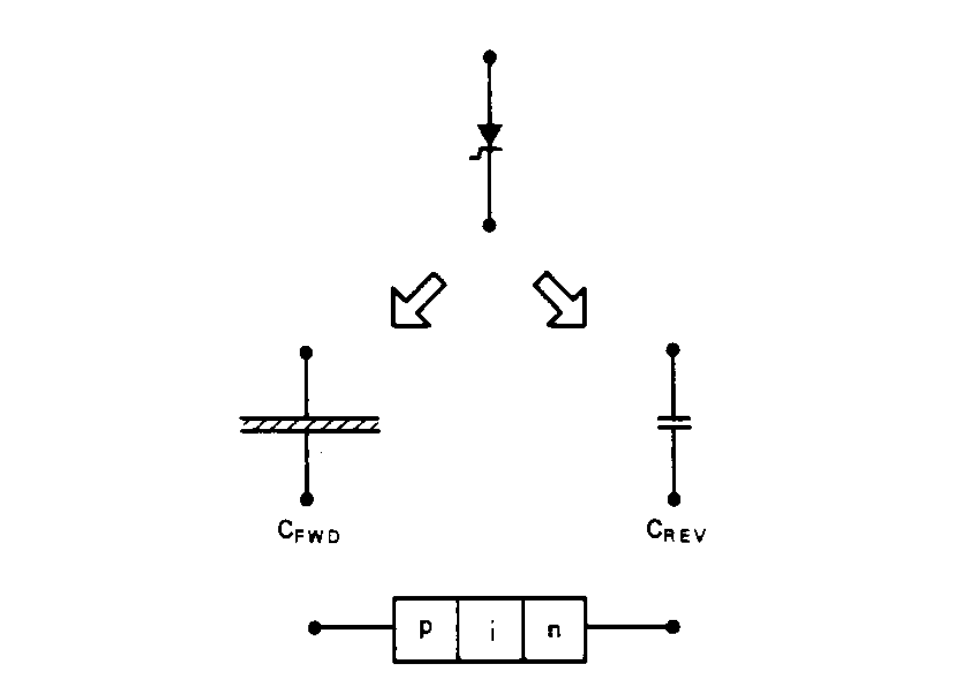
\includegraphics[width=\textwidth]{images/srd_switched_model.jpg}
        \caption{Modelo de capacidad conmutada del SRD. Tomada de
        \cite{moll1969}}
        \label{fig:srd_switched_model}
    \end{subfigure}
    \hfill
    \begin{subfigure}[b]{0.45\textwidth}
        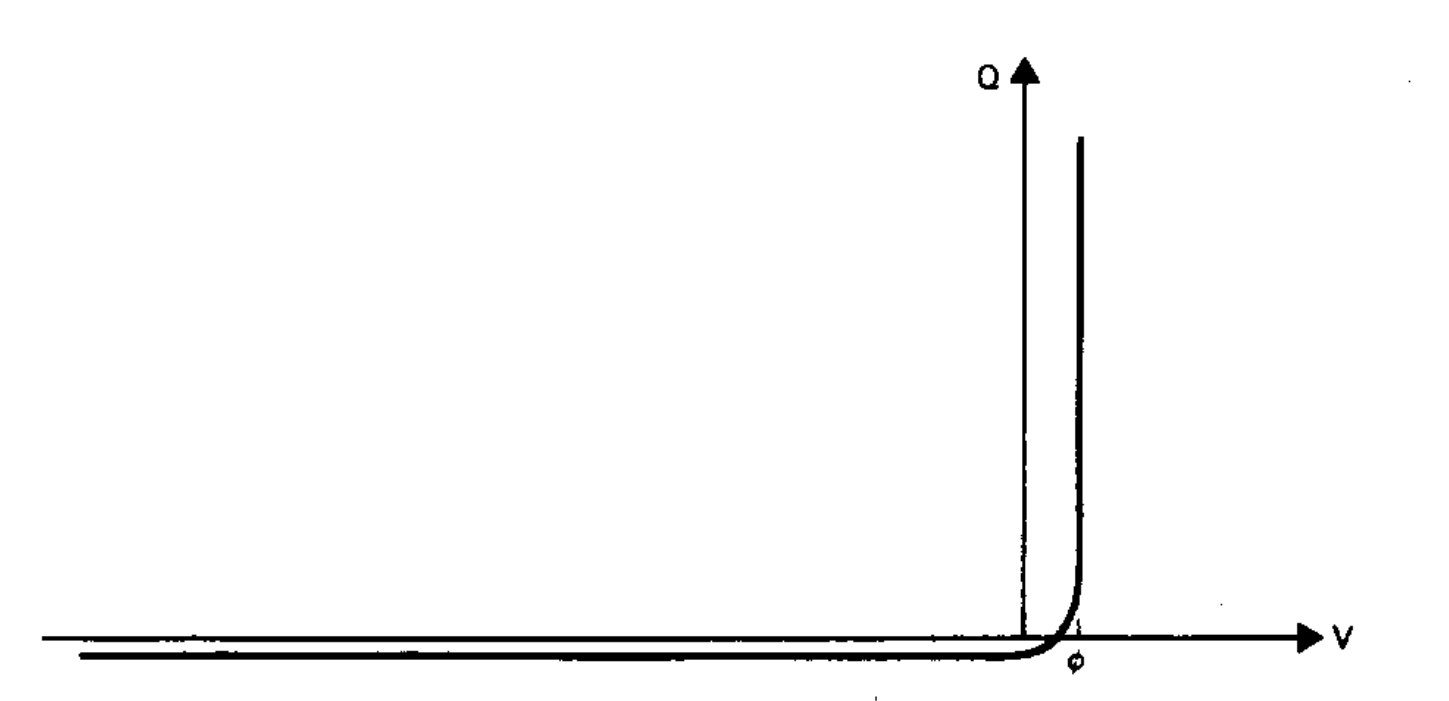
\includegraphics[width=\textwidth]{images/srd_capacity_vs_voltaje.jpg}
        \caption{Característica de capacidad en función de tensión para SRD.
        Tomada de \cite{moll1969}}
        \label{fig:srd_capacity_vs_voltaje}
    \end{subfigure}
    \caption{Características del modelo de SRD.}
    \label{fig:srd_model_characteristics}
\end{figure}

Para simular el diodo SRD, se utilizó un modelo de spice basado en este modelo
de capacidad de dos estados \cite{zhang1995} \cite{zhang1996}. Este modelo, que
puede observarse en la figura \ref{fig:srd_circuit_model}, está basado en un
modelo de capacidad conmutada en paralelo con una juntura PN.

Un problema del modelo de capacidad de la figura
\ref{fig:srd_capacity_vs_voltaje}, es la discontinuidad de la curva y su
derivada. Para mejorar este aspecto y tener un modelo utilizable en simuladores
comerciales, en \cite{zhang1995} se propone una mejora, Para modelar al
capacitor no lineal, se propone una relación entre carga y tensión lineal en 3
tramos, con valores que vuelven continua la curva y sus derivadas.

\begin{equation}
Q(V) =
    \left\{
    \begin{aligned}
        & C_r \cdot V  & V \leq 0 \\
        & c \cdot \left(V+a \right)^2 -b  & 0 < V < \phi \\
        & C_f \cdot \left( V - \phi \right) + Q_{rmp} & V \geq \phi \\
    \end{aligned}
    \right.
\end{equation}

En este modelo, la capacidad tiene un valor $C_r$ para valores de tensión
negativos, y $C_f$ para valores de tensión positivos. En el punto $V=\phi$, la
carga almacenada es $Q_{rmp}$, representando la carga residual en la juntura al
comienzo de la rampa de tensión descripta en la sección \ref{sec:srd_diode}.
Para la zona $0 < V < \phi$ se agregan constantes $a$, $b$ y $c$ para lograr una
curva continua. Se aplican las siguientes condiciones de contorno

\begin{equation}
    \left\{
    \begin{aligned}
        & Q(\phi) = Q_{rmp} \\
        & \frac{dQ}{dV}(\phi) = C_f \\
        & Q(0) = 0 \\
        & \frac{dQ}{dV}(0) = C_r \\
    \end{aligned}
    \right.
\end{equation}

Aplicando las condiciones de contorno, se llega a la siguiente relación

\begin{equation}
\label{eq:srd_non_linear_cap}
Q(V) =
    \left\{
    \begin{aligned}
        & C_r \cdot V  & V \leq 0 \\
        & \frac{C_f-C_r}{2\phi} \cdot \left(V+\frac{C_r\phi}{C_f-C_r} \right)^2
        -\frac{C_r^2}{2\left(C_f-C_r \right)}\cdot \phi  & 0 < V < \phi \\
        & C_f \cdot V - \frac{C_f-C_r}{2} \phi & V \geq \phi \\
    \end{aligned}
    \right.
\end{equation}

Para implementar esta capacidad no lineal, se necesitan los siguientes
parámetros:

\begin{itemize}
    \item $C_r$: esta es la capacidad de juntura del diodo, y es parte de las
        especificaciones del fabricante.
    \item $\phi$: es el potencial de juntura del diodo, especificado por el
        fabricante
    \item $C_f$: es la capacidad en directa del diodo. Se relaciona con el
        tiempo de vida de los portadores minoritarios $\tau_m$ y una resistencia
        dinámica $R_f$ a través de $\tau_m = C_f \cdot R_f$.
        \cite{Kotzebue1965}
\end{itemize}

La capacidad no lineal descripta en \ref{eq:srd_non_linear_cap} puede ser
implementada entonces con los datos provistos por el fabricante, solo siendo
necesario realizar una medición de la resistencia dinámica $R_f$. El modelo de
simulación final puede observarse en la figura \ref{fig:srd_circuit_model}.

En cuanto al alcance del modelo, este no contempla el tiempo de transición $t_t$
del diodo, por lo que sus efectos no están incluidos. Este modelo es suficiente
para análisis que involucren la carga y descarga del diodo, es decir, su
transición al estado de alta impedancia. El modelo no provee información sobre
la forma de esa transición.

Con esta curva se puede implementar el modelo de capacidad conmutada descripto
en \cite{moll1969} en una manera manejable para los simuladores de circuitos.
Bajo este modelo, se reportan en la literatura múltiples diseños de generadores
de pulsos \cite{Ruengwaree2006} \cite{Rahman2022} y multiplicadores de
frecuencia \cite{zhang1996} \cite{Heymann2001}, con buen acuerdo entre
simulación y medición.

Existen otros modelos de simulación para el diodo SRD, como los reportados en
\cite{Opalska1997} y \cite{Shevchenko2022} basados en balance de cargas. Sin
embargo, estos son más complejos en su implementación, ya que requieren
múltiples fuentes controladas y mediciones de diversos parámetros del diodo. Es
por esto que se utilizó el modelo de \cite{zhang1995}.

\begin{figure}[t]
  \centering
    \begin{circuitikz}[scale=0.8, transform shape]
    \node[spdt, rotate=-90] (sw) {};
        \draw   (sw.in)     node[above] {}   to [short] ++ (1,0) coordinate
        (aux1)
        (sw.out 1)  node[below] {}   to [short] ++ (+0.2,0) to [C, l=$C_r$] ++
        (0,-2) coordinate (aux2)
        (sw.out 2)  node[below] {}   to [short] ++ (-0.2,0) to [C, l_=$C_f$] ++
        (0,-2) |- (aux2);
        \draw (aux1) to[short] ++ (0.5,0)
                     to [short] ++ (0.5,0)
                     to [short] ++ (0,-1)
                     to[D, l=$D$] ++ (0,-1) |- (aux2);
        \draw (aux2) to[short] ++ (0.4,0) to [short] ++ (0,-0.5)
                     to [R=$R_s$] ++ (0,-1.5)
                     to [L=$L_p$] ++ (0,-2) coordinate (aux3);
        \draw (aux1) to[short] ++ (0,1) coordinate (aux4);
        \draw (aux4) to[short] ++ (2,0) to[C=$C_p$] ++ (0,-8) |- (aux3);
        \draw (aux4) to[short, -o] ++ (-3,0) coordinate (aux5);
        \draw (aux5) to[open, i^=$I_D$] (aux4);
        \draw (aux3) to[short, -o] ++ (-3,0)
                     to[open, v^=$V_D$, european,] (aux5);
    \end{circuitikz}
    \caption{Modelo de simulación del SRD.}
    \label{fig:srd_circuit_model}
\end{figure}

\section{Selección de SRD}

Para la implementación del generador de pulsos de este trabajo se seleccionó un
diodo SRD MMD830 de MACOM \cite{mmd830-datasheet}. Este pertenece a la familia
de diodos SRD MMDx.  Dentro de la familia hay diversos modelos con métricas de
desempeño proporcionales a su precio. En la tabla \ref{tab:mmdx_performance} se
muestran algunos dispositivos de la familia.

Se decidió este diodo por un balance entre desempeño y costo. Al momento de su
adquisición, en agosto de 2022, el mismo tenía un costo de USD 54. Al momento de
la redacción de este trabajo, el costo del mismo es de USD 33. La gran variación
se debió al faltante de semiconductores que se experimentó en ese momento. El
dispositivo tiene un costo elevado a comparación de semiconductores usuales que
están en el rango de .1-5 USD, pero no deja de ser un valor aceptable para la
implementación de una plataforma de bajo costo.

La familia viene en distintos tipos de encapsulados. Los hay desde \textit{bare
die} y \textit{beam lead} hasta plástico, cerámico o vidrio. Dado los distintos
parásitos que cada encapsulado tiene, tanto por su material como por su tamaño,
el desempeño de los dispositivos presenta grandes variaciones. Por ejemplo, el
tiempo de transición $t_t$ más rápido de todos es de \qty{30}{\pico\second},
para el MMDB30-B11 en en \textit{beam lead}. Este presenta una capacidad de
juntura de \qty{0.20}{\pico\farad} y una tensión de ruptura de \qty{14}{\volt}.
En el otro extremo, el más lento de todos es el MMD0803 en encapsulado de
vidrio, con un tiempo de transición de \qty{400}{\pico\second}, capacidad total
de \qty{6.15}{\pico\farad}, y tensión de ruptura de \qty{70}{\volt}. Estas
relaciones son consistentes y predecibles por el modelo teórico del
funcionamiento físico de los dispositivos presentado en la sección
\ref{sec:srd_diode}.

Entre los distintos encapsulados, se mantienen las figuras de tiempo de vida de
portadores $\tau_m$ y tiempo de transición $t_t$ para los mismos modelos. Lo que
cambia con el encapsulado, es la capacidad total $C_T$, incrementando con
mayores tamaños de encapsulado y resultando en una menor frecuencia de corte.

\begin{table}[t]
\centering
\begin{tabular}{|c|c|c|c|c|c|c|c|}
\hline
    \multirow{2}{*}{Modelo} & $V_B$ [V] &
    \multicolumn{2}{c|}{$C_j$ [pF]} & \multicolumn{2}{c|}{$\tau_m$ [ns]} &
    \multicolumn{2}{c|}{$t_t$ [ps]} \\
\cline{2-8}
    & Min & Min & Max & Min & Typ & Typ & Max \\
\hline
MMD805-0805-2 & 60 & 2.56 & 3.56 & 80 & 100 & 250 & 300 \\
MMD810-0805-2 & 50 & 1.75 & 2.75 & 40 & 70  & 200 & 250 \\
MMD820-0805-2 & 40 & 1.06 & 1.76 & 30 & 60  & 80  & 100 \\
MMD830-0805-2 & 25 & 0.56 & 1.06 & 15 & 30  & 60  & 80 \\
MMD832-0805-2 & 20 & 0.46 & 0.86 & 10 & 15  & 60  & 80 \\
MMD835-0805-2 & 15 & 0.36 & 0.86 & 10 & 20  & 50  & 70 \\
\hline
\end{tabular}
\caption{Desempeño de familia de SRD MMDx de MACOM.}
\label{tab:mmdx_performance}
\end{table}

El encapsulado elegido es uno cerámico, el 0805-2. En la figura
\ref{fig:srd_0805_outline} puede observarse un diagrama del mismo, con sus
dimensiones en mils y mm. Es un encapsulado muy pequeño, de
\qty{2.16}{\milli\meter} por \qty{1.40}{\milli\meter}. En la hoja de datos se
especifican su capacidad $C_p$ e inductancia $L_p$ parásitas en
\qty{0.06}{\pico\farad} y \qty{0.4}{\nano\henry} respectivamente.

\begin{figure}[t]
  \centering
    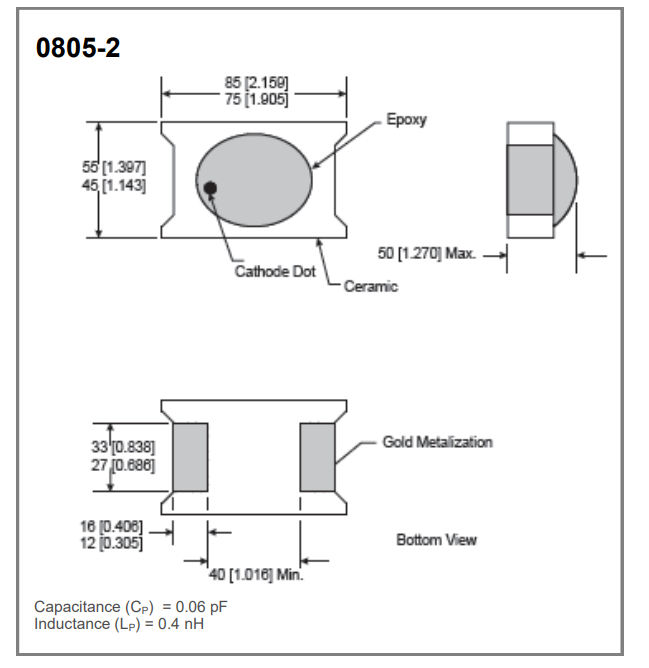
\includegraphics[width=0.4\textwidth]{images/srd_0805_outline.jpg}
    \caption{Dimensiones del encapsulado utilizado.}
    \label{fig:srd_0805_outline}
\end{figure}

\subsection{Validación de modelo}

Para validar el modelo propuesto para el SRD, y comprobar el desempeño del diodo
seleccionado, se realizaron simulaciones en el software ADS. Para el modelo se
utilizó el descripto en la sección \ref{sec:srd_simulation_models} y presentado
en \cite{zhang1995}.

En la figura \ref{fig:srd_model_ads} se observa el modelo implementado para el
SRD. El mismo contiene las inductancias y capacidad parásitas del encapsulado
$C_p$ y $L_p$.

\begin{figure}[t]
  \centering
    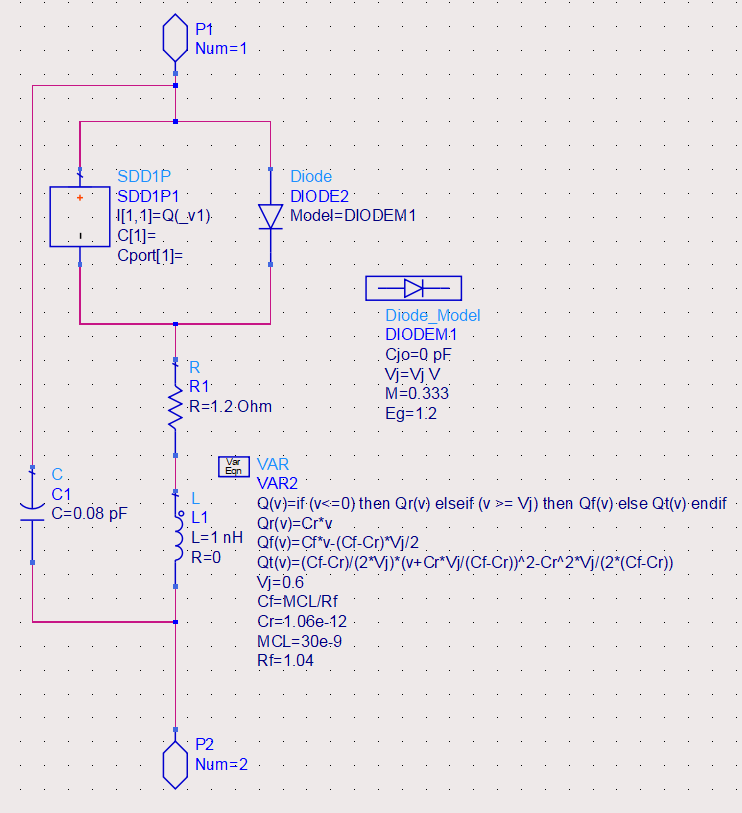
\includegraphics[width=0.4\textwidth]{images/srd_model_ads.jpg}
    \caption{Modelo implementado en ADS para el SRD.}
    \label{fig:srd_model_ads}
\end{figure}

Para modelar al diodo en sí, se colocan en paralelo una juntura PN y un
dispositivo definido simbólicamente. Este es un tipo de dispositivos disponibles
en ADS que permiten definir una relación arbitraria entre las variables del
dispositivo. En este caso, se define una relación entre la carga $Q(t)$ y la
tensión $v(t)$, definiendo de esta manera un capacitor no lineal. El capacitor
definido es el descripto en la sección \ref{sec:srd_simulation_models} y
presentado en \cite{zhang1995}.

Como el capacitor no lineal definido contempla tanto la capacidad de difusión
como la capacidad de juntura del diodo, en el modelo de diodo utilizado para
modelar la juntura, se define una capacidad de juntura de \qty{0}{\pico\farad},
para evitar modelar dos veces la misma. De esta manera, la juntura únicamente
modela la relación IV del diodo, $i_D(t) = I_S \left(
e^{\frac{v_D(t)}{V_T}}-1\right)$.

\subsection{Simulación}

Con el modelo de SRD definido, se valida su comportamiento con una simulación.
En la figura \ref{fig:srd_validation_schematic} puede observarse el circuito
simulado. Consiste de una fuente de tensión en serie con el SRD y una
resistencia de limitación de corriente. Se simula el escenario dos veces con
estímulos distintos: una señal cuadrada y una senoidal, ambas de
\qty{10}{\mega\hertz} de frecuencia, \qty{10}{\volt} de amplitud pico-a-pico y
\qty{0}{\volt} de valor medio.

\begin{figure}[t]
  \centering
    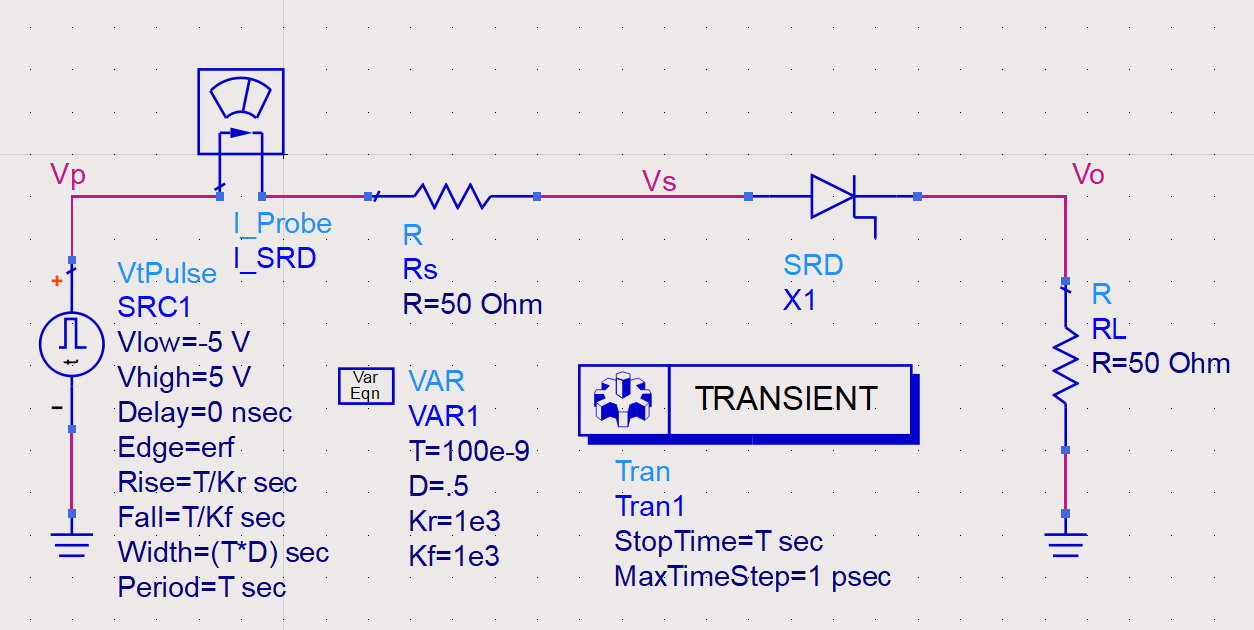
\includegraphics[width=0.4\textwidth]{images/srd_validation_schematic.jpg}
    \caption{Esquemático de simulación de modelo de SRD.}
    \label{fig:srd_validation_schematic}
\end{figure}

En la figura \ref{fig:srd_results} pueden observarse los resultados. En ambos
casos, para entrada senoidal y cuadarada, dado que no hay elementos resonantes,
corriente y tensión están en fase. En ambos ejes se observan las escalas. En
ambos casos, se observa como la salida sigue a la entrada, afectada por el
divisor de tensión de $R_L$ y $R_s$. Una vez que la corriente cambia el signo y
toda la carga del SRD es removida, este transiciona al estado de alta
impedancia, colapsando rápidamente la tensión a \qty{0}{\milli\ampere} y la
tensión de salida a \qty{0}{\volt}.

\begin{figure}
    \centering
    \begin{subfigure}[b]{0.45\textwidth}
        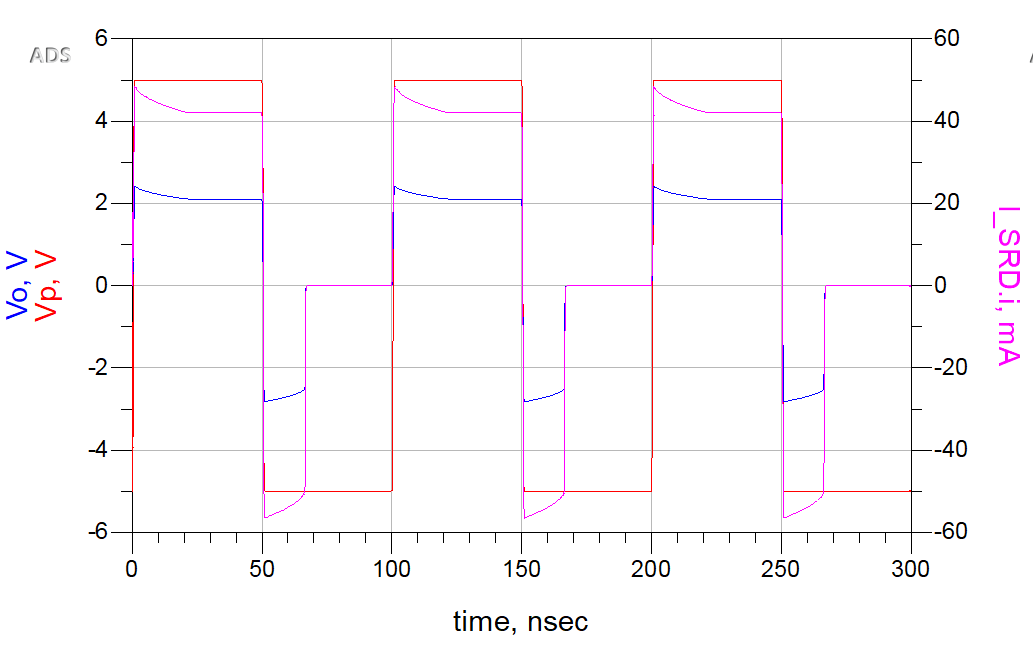
\includegraphics[width=\textwidth]{images/srd_result_square.png}
        \caption{Resultado de simulación con entrada cuadrada.}
        \label{fig:srd_result_square}
    \end{subfigure}
    \hfill
    \begin{subfigure}[b]{0.45\textwidth}
        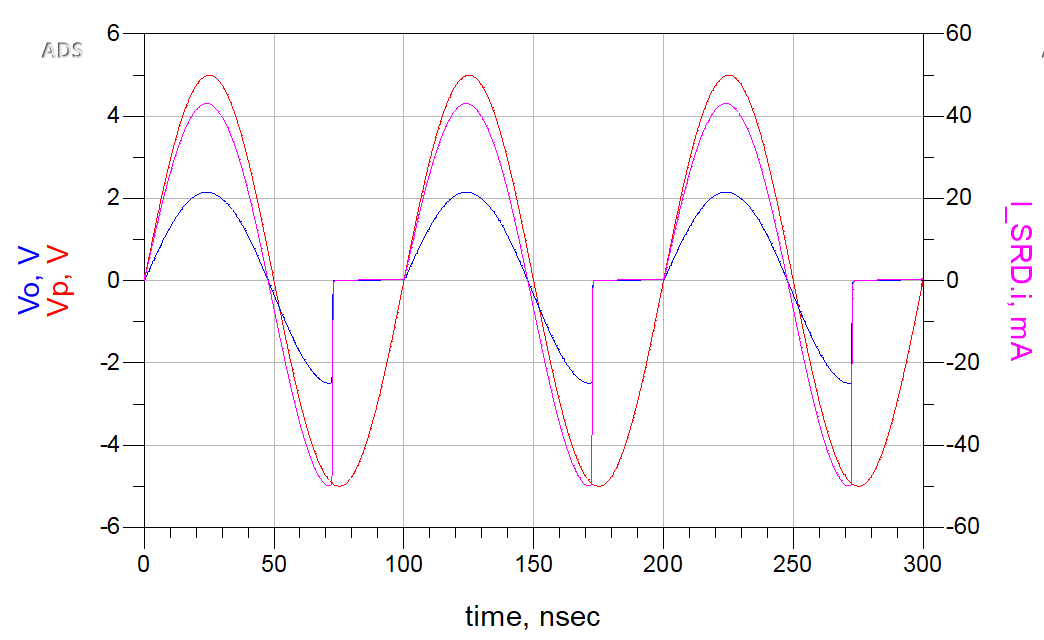
\includegraphics[width=\textwidth]{images/srd_result_sine.png}
        \caption{Resultado de simulación con entrada senoidal.}
        \label{fig:srd_result_sine}
    \end{subfigure}
    \caption{Resultados de simulación de modelo de SRD.}
    \label{fig:srd_results}
\end{figure}

Como fuese explicado en la sección \ref{sec:srd_simulation_models}, el modelo
utilizado contempla el tiempo de vida de los portadores minoritarios $\tau_m$,
pero no el tiempo de transición $t_t$. Por lo tanto, de estas simulaciones se
espera un correcto modelado del tiempo de almacenamiento $t_s$ pero no del
tiempo de crecimiento de la señal una vez terminado el tiempo de almacenamiento.

El tiempo de crecimiento de la señal dependerá tanto del tiempo de transición
del diodo $t_t$ como del circuito, a través de una constante de tiempo $t_{RC}$.
Si $R$ y $C$ son la resistencia y capacidad entre los terminales del SRD, el
tiempo de crecimiento $t_r$ será \cite{an918}

\begin{equation}
    t_r = \sqrt{t_t^2+t_{RC}^2}
\end{equation}

La capacidad $C$ estará compuesta por la capacidad de juntura del diodo y todas
las capacidades parásitas (de encapsulado y de PCB) que se encuentren. En la
simulación realizada, $t_t$ es nulo, por lo que el tiempo de crecimiento $t_r$
observado es igual a $t_{RC}$. En esta simulación la única capacidad es la de
juntura, en una simulación con extracción de parásitos, se contemplarían las
capacidades de las estructuras adyacentes.
